\section{Motivating Examples}\label{sec:example}

The goal of using an automated random testing tool is to test code without effort in a 
short amount of time and discover faults that may otherwise go unnoticed.
To show how our approach can be used, we present a small motivating example.
Imagine that one wants to code a class that represents integers and some of their operators.
A very simple version of the class could be:

{\small
\begin{verbatim}
public class MyInteger {
  int value;
  public MyInteger(int val){
    value = val;
  }
  public int intValue(){
    return value;
  }
  public void square(){
    value = value*value;
  }
  public boolean isDivisibleBy(MyInteger divisor){
    int other = divisor.intValue();
    if (((value/other)*other)==value)
      return true;
    return false;
  }
}
\end{verbatim}
}

Such a simple class already contains a number of faults that are typically forgotten by programmers.
To find faults in this code, we can use YETI for 1 second:
{\small
\begin{verbatim}
java -ea -Java -testModules=MyInteger -time=1s -randomPlus
\end{verbatim}
}

YETI then generates automatically instances on-demand and keeps a bounded number of them in the system in order to reuse them for future calls. 
Generating an instance is made through constructors and recursive calls to the constructors of types of arguments of the constructors. 
When a method is called, the result is also added to the instances usable by subsequent calls.

At the end of the testing session, the tool generates both a report and test cases reproducing the two faults found (a division by 0 and a dereferencing of a null pointer):
{\small
\begin{verbatim}
@Test public void test_1() throws Exception {
  int v0=1; // time:1297437861978
  MyInteger v8=new MyInteger(v0); // time:1297437861980
  boolean v21=v8.isDivisibleBy(null); // time:1297437861982
  /**BUG FOUND: RUNTIME EXCEPTION**/ // time:1297437861983
  /**YETI EXCEPTION - START 
  java.lang.NullPointerException
    at MyInteger.isDivisibleBy(MyInteger.java:13)
  YETI EXCEPTION - END**/ 
  /** original locs: 25 minimal locs: 3**/
}
@Test public void test_2() throws Exception {
  int v258=6; // time:1297437862051
  MyInteger v259=new MyInteger(v258); // time:1297437862051
  int v509=0; // time:1297437862120
  MyInteger v510=new MyInteger(v509); // time:1297437862120
  boolean v511=v259.isDivisibleBy(v510); // time:1297437862121
  /**BUG FOUND: RUNTIME EXCEPTION**/ // time:1297437862122
  /**YETI EXCEPTION - START 
  java.lang.ArithmeticException: / by zero
    at MyInteger.isDivisibleBy(MyInteger.java:14)
  YETI EXCEPTION - END**/ 
  /** original locs: 607 minimal locs: 6**/
}
/** Non-Unique bugs: 32, Unique Bugs: 2, Logs size (locs): 2443**/
/** Testing Session finished, number of tests:2298, time: 1007ms , 
    number of failures: 36**/
/** Processing time: 11ms **/
/** Branch coverage: 6/6(100.0%) **/
/** Testing finished **/
\end{verbatim}
}

More faults exist in this program, but without specifications, we cannot find them in an automated way.
If we add some specifications -- even incomplete ones -- we then find more faults using exactly the same tool.
For example, adding \verb+assert value>0;+ at the end of \verb+square+ uncovers one more fault:

{\small
\begin{verbatim}
@Test public void test_3() throws Exception {
  int v40=151060480; // time:1297439368019
  MyInteger v78=new MyInteger(v40); // time:1297439368025
  v78.square(); // time:1297439368025
  /**BUG FOUND: RUNTIME EXCEPTION**/ // time:1297439368026
  /**YETI EXCEPTION - START 
  java.lang.AssertionError
    at MyInteger.square(MyInteger.java:11)
  YETI EXCEPTION - END**/ 
  /** original locs: 97 minimal locs: 3**/
}
\end{verbatim}
}

While there are still faults in the program -- and some can be found using YETI by writing more precise specifications --, we can see that we already found 3 faults that might prove critical in an application using this simple class (for example, an overflow was at the core of the Ariane 5 incident,\footnote{\url{http://esamultimedia.esa.int/docs/esa-x-1819eng.pdf}} and division by 0 in the USS Yorktown incident\footnote{\url{http://www.wired.com/science/discoveries/news/1998/07/13987}}).

\subsection{Graphical User Interface (GUI)}
One of the main issues when using a command-line testing tool is that it is usually 
difficult to diagnose whether a testing session is performing as scheduled. 
In particular, automated random testing might generate large amounts of data which might lead to 
poor performances. 
As it is not convenient to discover the problem only at the end of the testing session, 
we added a graphical user interface to YETI in order to give users more control on the testing process.
 
%By specifying the \texttt{-gui} option, YETI has a graphical user interface
%that allows test engineers to interact directly with the system while the testing 
%session proceeds. 
%
\begin{sidewaysfigure}
%\begin{figure}[ht]
%\begin{center}
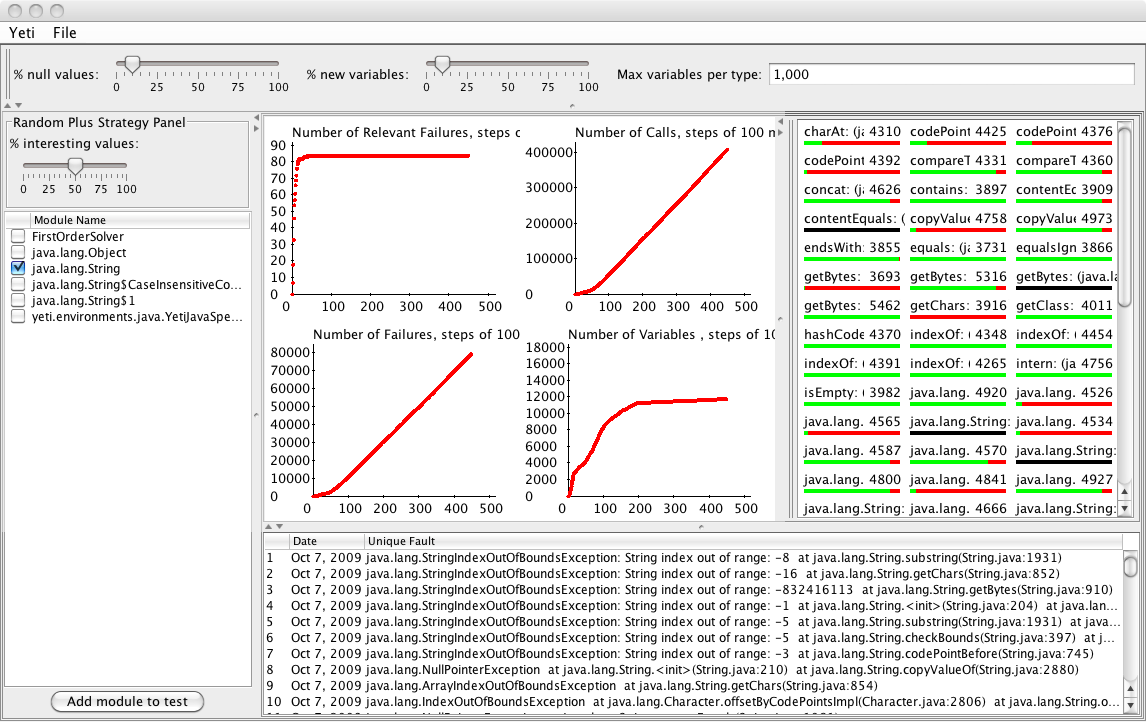
\includegraphics[width=20cm]{images/YetiComplete.png}
%\end{center}
\caption{YETI graphical user interface.}\label{fig:gui}
%\end{figure}
\end{sidewaysfigure}

Figure~\ref{fig:gui} shows YETI's graphical user interface when using 
the random+ strategy. At the top left of the interface, two sliders correspond to 
the percentage of null values and the percentage of new variables to use when testing.
Each time a test is made, each parameter of the routine to test can either 
be void, newly generated or a new variable. These sliders indicate which probability 
to use. In the top part there is also a text field to limit the number of instances per 
type in the system (which is necessary for long-running sessions).

The left panel contains a subpanel specific to the current strategy (in the example, it 
considers how to use ``interesting'' values when possible) and a list of modules loaded in 
the system. The modules being tested are ticked, while others can be used as helpers to 
create variables on demand when making a routine calls. A button is available to add modules 
at runtime for programming languages that support it. This last part is useful in cases 
where a module is missing for testing a routine. 

In the central panel, four graphs describe the evolution of the system over time: the top-left one shows 
the evolution of the number of unique failures found -- all failures without redundancy --, the 
bottom-left indicates the raw number of failures over time, the bottom-right indicates the current 
number of instances in the system, the top-right panel indicates the total number of calls effected by YETI.

The panel on the right shows all methods tested in the system and presents results in the form 
of a colored gauge where black indicates that the routine was not tested, green is the proportion
of routines tested successfully, yellow represents routine calls that cannot be interpreted
-- for example,	 YETI had to stop a thread --, and red indicates failures.
The bottom panel reports unique failures as they are found: each line is a unique failure.


\subsection{Reporting in Real-Time}

Other random testing tools do not include any way of interacting with the infrastructure in real-time.
YETI allows it and it benefits test engineers because they can adapt the testing process to fit their needs. 
To decide whether to stop testing, testers can now monitor the general evolution of the number of unique 
faults found. If the graph shows that no faults were found in the latest part of the testing session, it is likely 
that no more faults will be uncovered. 

We show two more scenarios where having real-time reporting in YETI allows test engineers to adapt and circumvent issues.

\paragraph{Using results from other techniques}
\begin{figure}[ht!]
{\small
\begin{verbatim}
// A class where random does not find 
// the bug unless very lucky
public class MyClass{
   public int div(int i){
      return i/(4556767-i);
   }
}
// Helper class to generate the interesting 
// value 4556767 in priority
public class HelpMyClass {
   public static int value(){
     return 4556767; 
   }
}
\end{verbatim}
}
\caption{A class to test.}\label{fig:myClass}
\end{figure}

Figure~\ref{fig:myClass} shows the code of \texttt{MyClass}, a class that only contains a method that calculates $i/(4556767-i)$ ($i$ being its argument). Obviously, passing $4556767$ as an argument will lead to a failure. When using a black-box random testing approach, for the tool to test the method with $4556767$ 
requires it to be lucky or to wait for a potentially long time for the testing to perform. 
In this particular case, to help YETI finding the fault, a software tester could create the class \texttt{HelpMyClass} (see Figure~\ref{fig:myClass}) that contains a method returning that value and load it at runtime.
%\begin{figure}[h!]
%\begin{center}
%\includegraphics[width=\columnwidth]{images/HelpMyClass.png}
%\end{center}
%\caption{Faults evolution when introducing HelpMyClass at 56s, \texttt{div} had been called $3\times10^{5}$ times out of $2\times10^{6}$ total calls.}\label{fig:helpmyclass}
%\end{figure}
After loading, the fault is then found immediately.
% (56s after the beginning of testing).

\paragraph{Testing untested methods and adapting the strategy at runtime}

One of the visible issues in Figure~\ref{fig:gui} is that the method \texttt{contentEquals} from \texttt{String} is not tested by YETI. The reason is that it uses instances of the class \texttt{StringBuffer} and even if the JVM knows it, YETI does not. The reason is that, for performance reasons, YETI does not load the whole transitive closure of types used in the tested program. The natural reaction in such a case is for the test engineer to add the module (load the class using the button in the lower-left part of the GUI). 

The issue is that \texttt{StringBuffer} is a buffer that can be initialized with a pre-defined capacity (an \texttt{int}). If numerous instances are initialized using large values, then the performances drop due to the large amount of memory needed by the JVM. A recovery strategy is to limit the number of instances per type and only keep a small number of them in the system.

\begin{figure*}[ht!]
\begin{center}
\includegraphics[width=\textwidth]{images/StringBuffer.png}
\end{center}
\caption{Testing \texttt{String}, adding \texttt{StringBuffer}, and then reducing the number of instances per type (in this case 2).}\label{fig:StringBuffer}
\end{figure*}

Figure~\ref{fig:StringBuffer} presents the graphs obtained in such a scenario. It is visible in the figure that introducing \texttt{StringBuffer} has a positive impact on the number of faults. It also impacts the performances. By reducing the number of instances per type we then improve the situation, which also allows YETI to find more faults.